\section{IoT system}
In this experiment, we have tested our approach on two IoT systems. First one is Power load leveling located in 102C2 room (From now on we call this IoT system eroom). Another IoT system is a smart electricity consumption meter implemented into the faculty of engineering Building 2 as a part of Tokyo Green project. (This device is located on the 10th, so we call it 10F)

\subsection{eroom}
Power load leveling is a system that usually found in renewable sources electricity generator. System’s function is to balance the energy, for example in solar panel case; it can store or sale the excessive electricity produced during daytime, while provide insufficient electricity during night. 

eroom an IoT system that connects power load levelling with battery, controller and air conditioners. Its functions are described below: 
\begin{enumerate}[itemsep=0mm]
    \item Commanding the power load leveling to either sale or store the excessive electricity.
    \item Providing stored electricity to the connected air conditioners. 
    \item Visualizing the electric consumption data on web server.
\end{enumerate}

\begin{figure}
    \centering 
    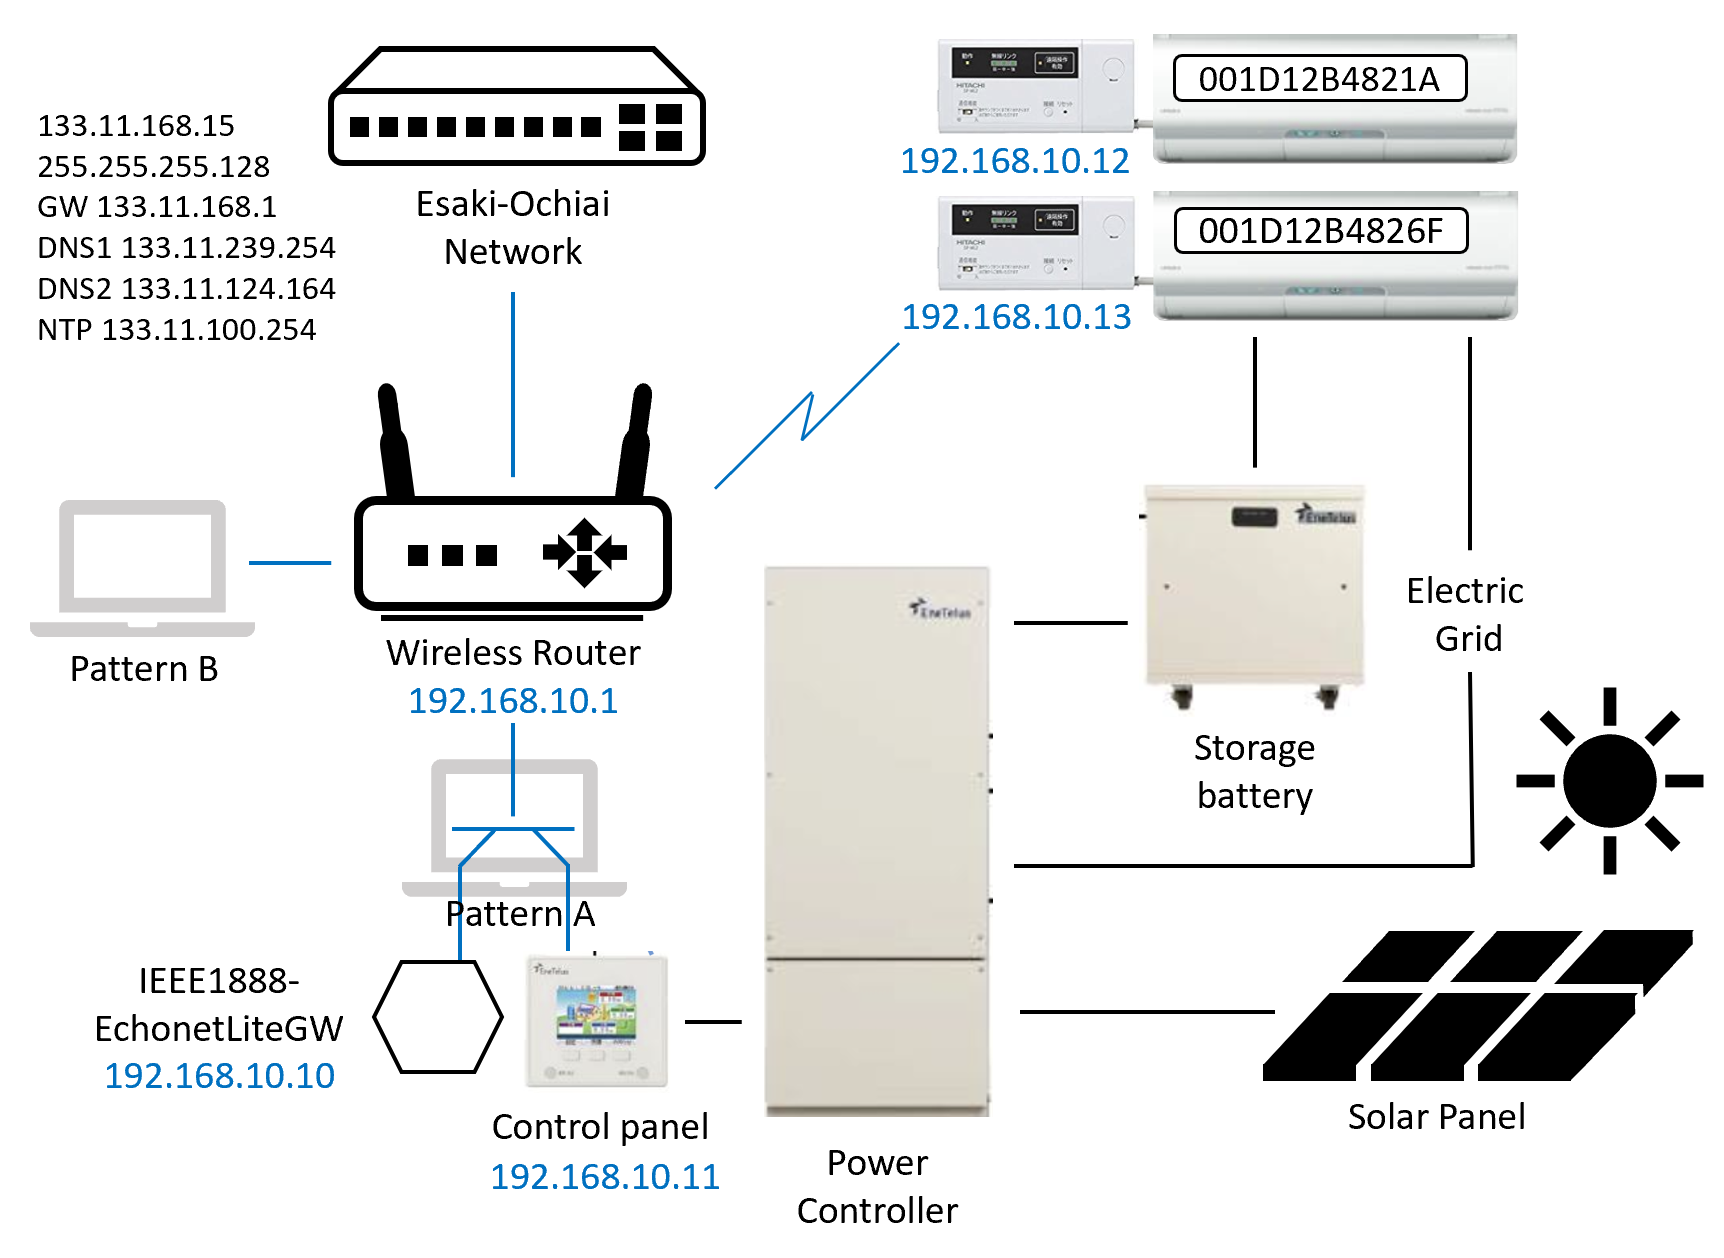
\includegraphics[width=0.7\textwidth]{4_eroom}
    \caption{\small The network topology of eroom.}
    \label{fig:s4_eroom}
\end{figure} 

The network topology of eroom IoT is shown in figure \ref{fig:s4_eroom}. 
Blue line indicates that devices is connected through ethernet cable, while black line represents the electrical cable. 
Devices are connected to the internet through the network of Esaki-Ochiai laboratory.
There are 4 IoT devices and a wireless router present in the system: 

\begin{itemize}[itemsep=0mm]
    \item The control panel (192.168.10.11)
    \item IEEE1888-EchonetLiteGW (192.168.10.10); 
    EchonetLite is communication protocol standard for devices used in smart hourse (air conditioner, lighting equipment or electricity sensor).
    IEEE1888-EchonetLiteGW is a middleware adapter. Its duty is to communicate with smart devices, in this case the air conditioners, and the control panel.
    \item 2 Air conditioners with controller (192.168.10.12, 192.168.10.13). 
    They are connected to 2 power supply: electric grid and battery.
    \item (Wireless Router (192.168.10.1) connecting all 4 devices and the internet)
\end{itemize}


\subsection{10F}

10F is a decentralized electric consumption visualization system. It collects electric usage data, 
then visualize it on the web server. Figure \ref{fig:s4_10f} shows architecture of this IoT system. 

\begin{figure}[H]
    \centering 
    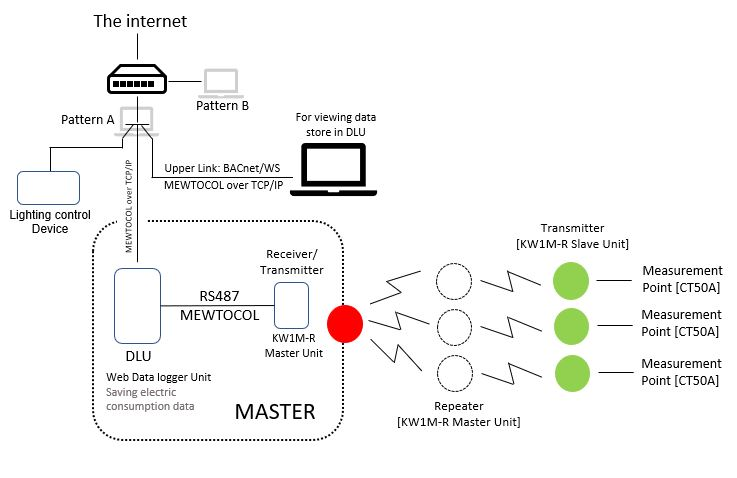
\includegraphics[width=0.7\textwidth]{4_10f}
    \caption{\small The architecture of 10F.}
    \label{fig:s4_10f}
\end{figure} 



The system is consisted of measurement unit, slave transmitter, repeater, master transmitter and Web Datalogger Unit (UDL).  

\begin{figure}[h]
    \centering
    \begin{subfigure}[b]{0.3\textwidth}
        \centering
        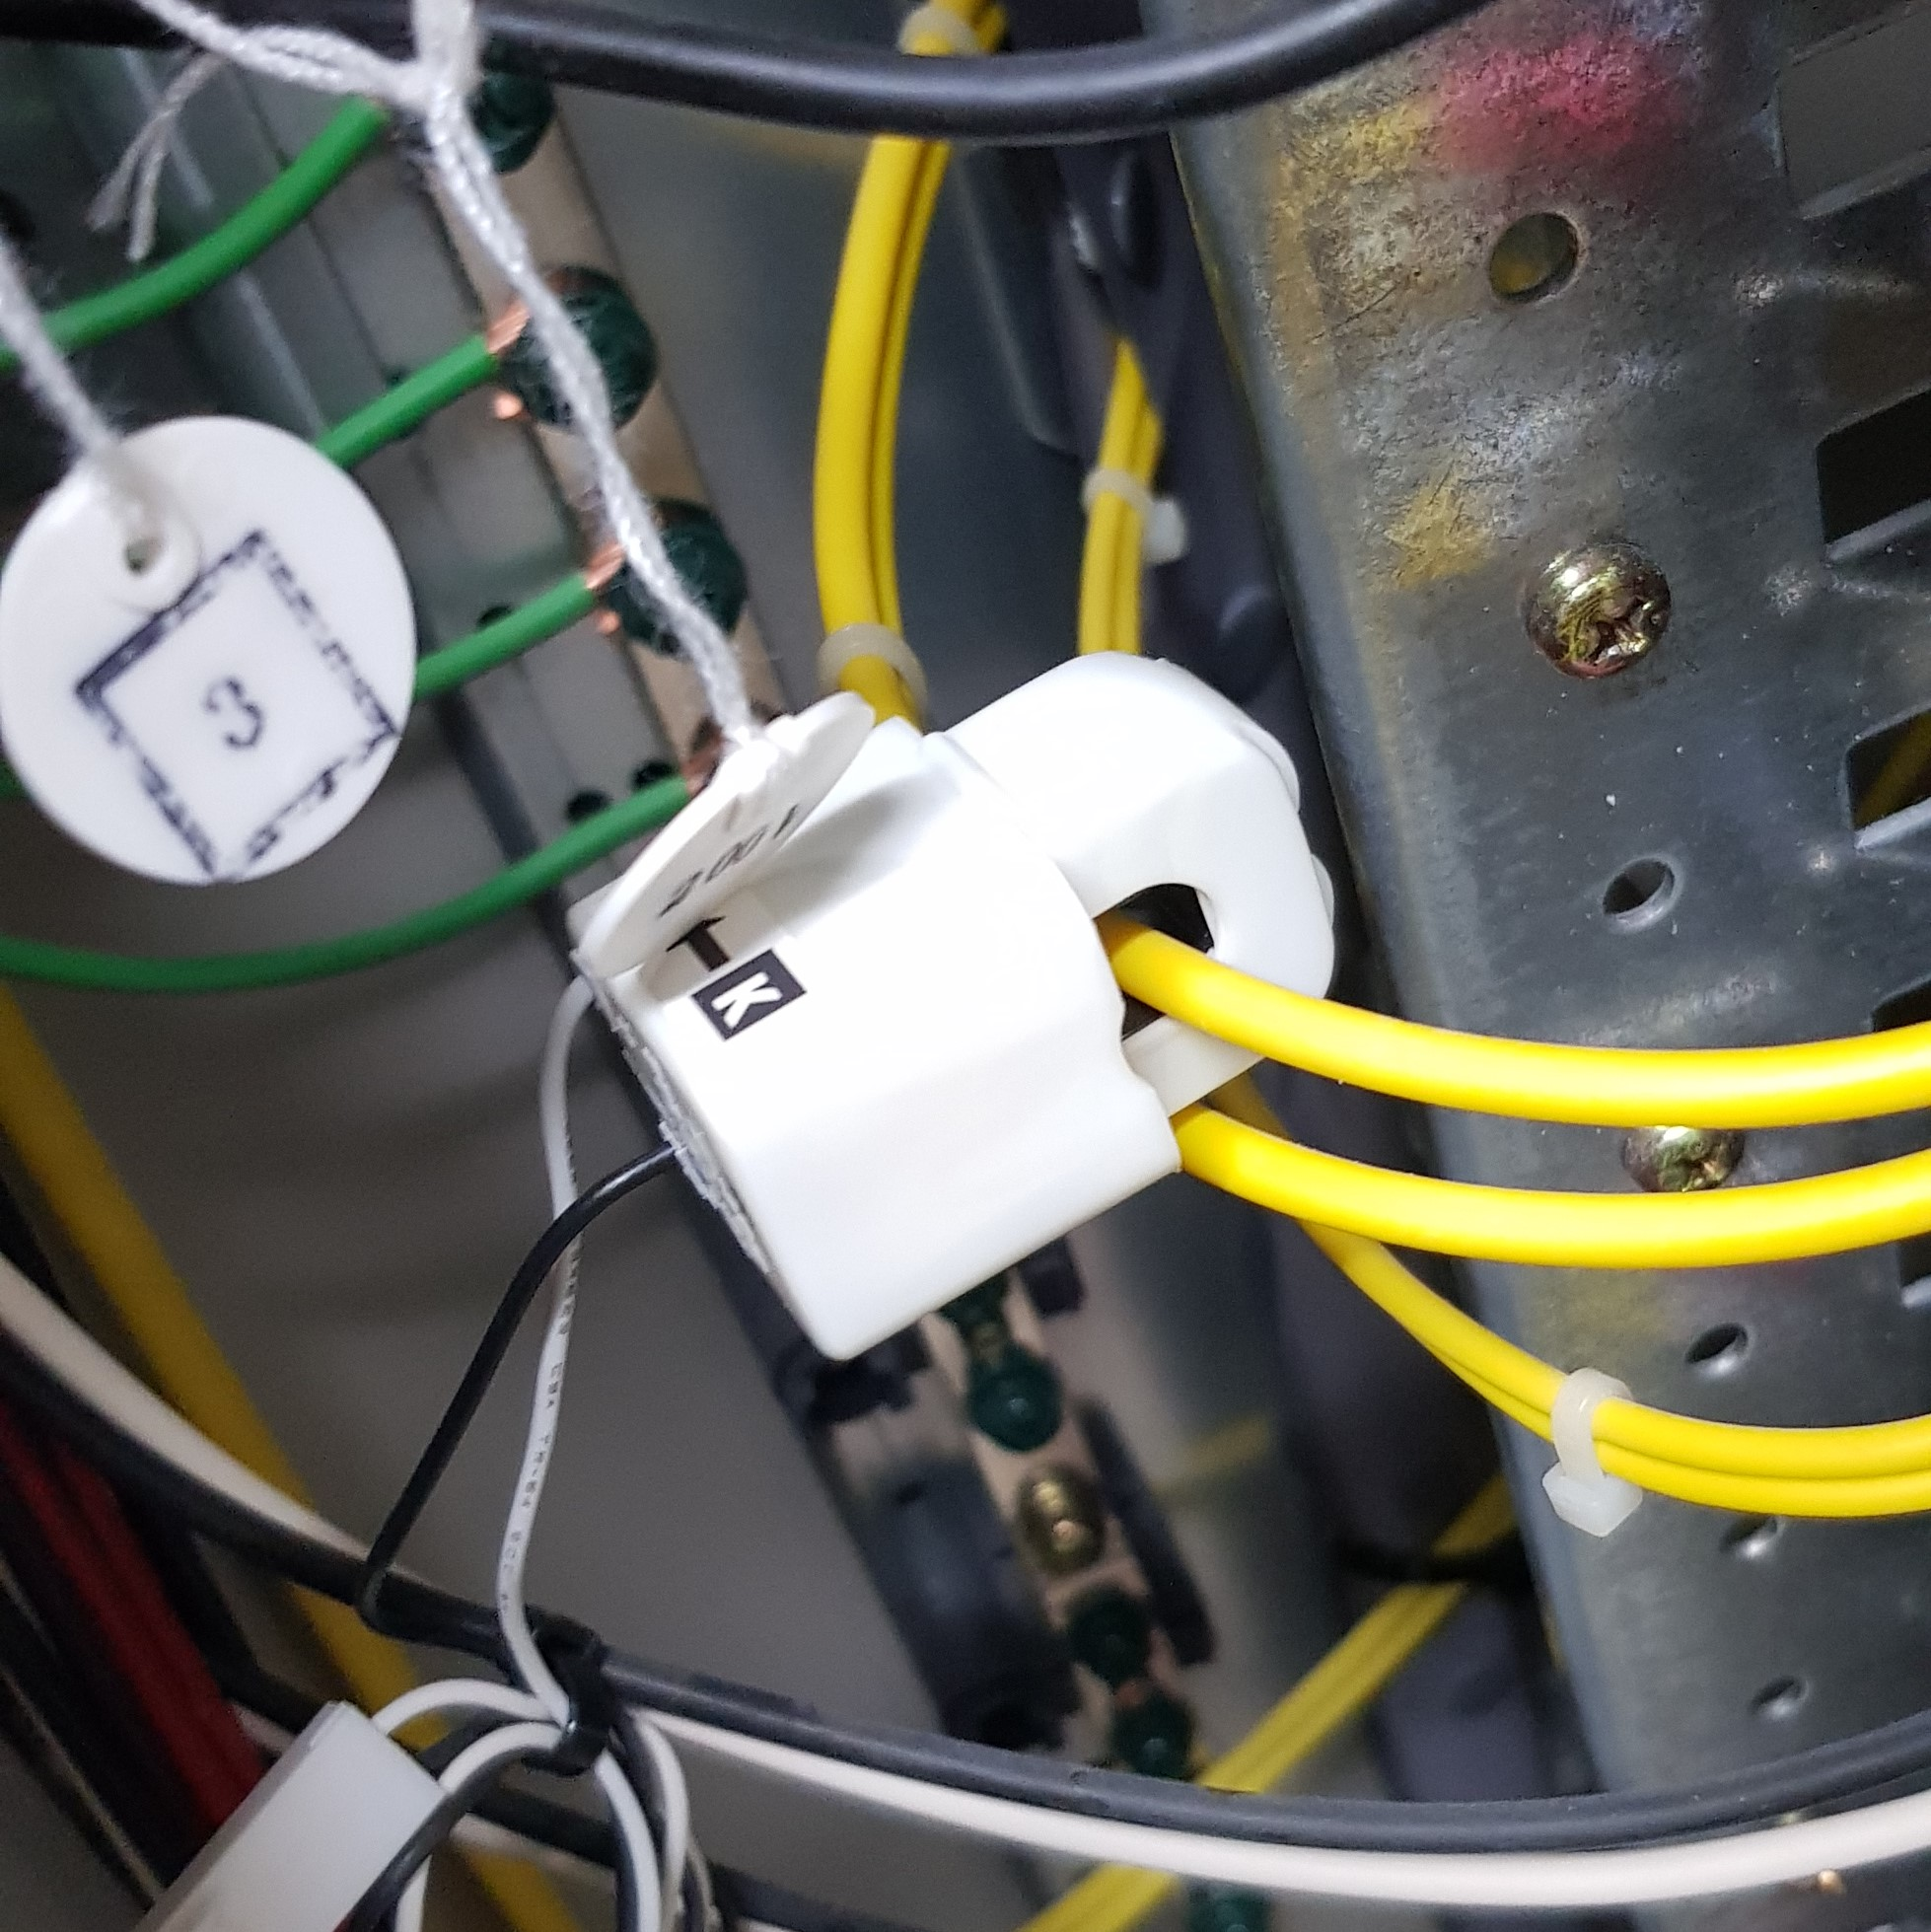
\includegraphics[width=\textwidth]{10f/1_1_measure_unit}
        \caption{\small CT50A Measurement unit (10F EPS-4)}
        \label{fig:s4_measure}
    \end{subfigure}
    \hfill
    \begin{subfigure}[b]{0.3\textwidth}
        \centering
        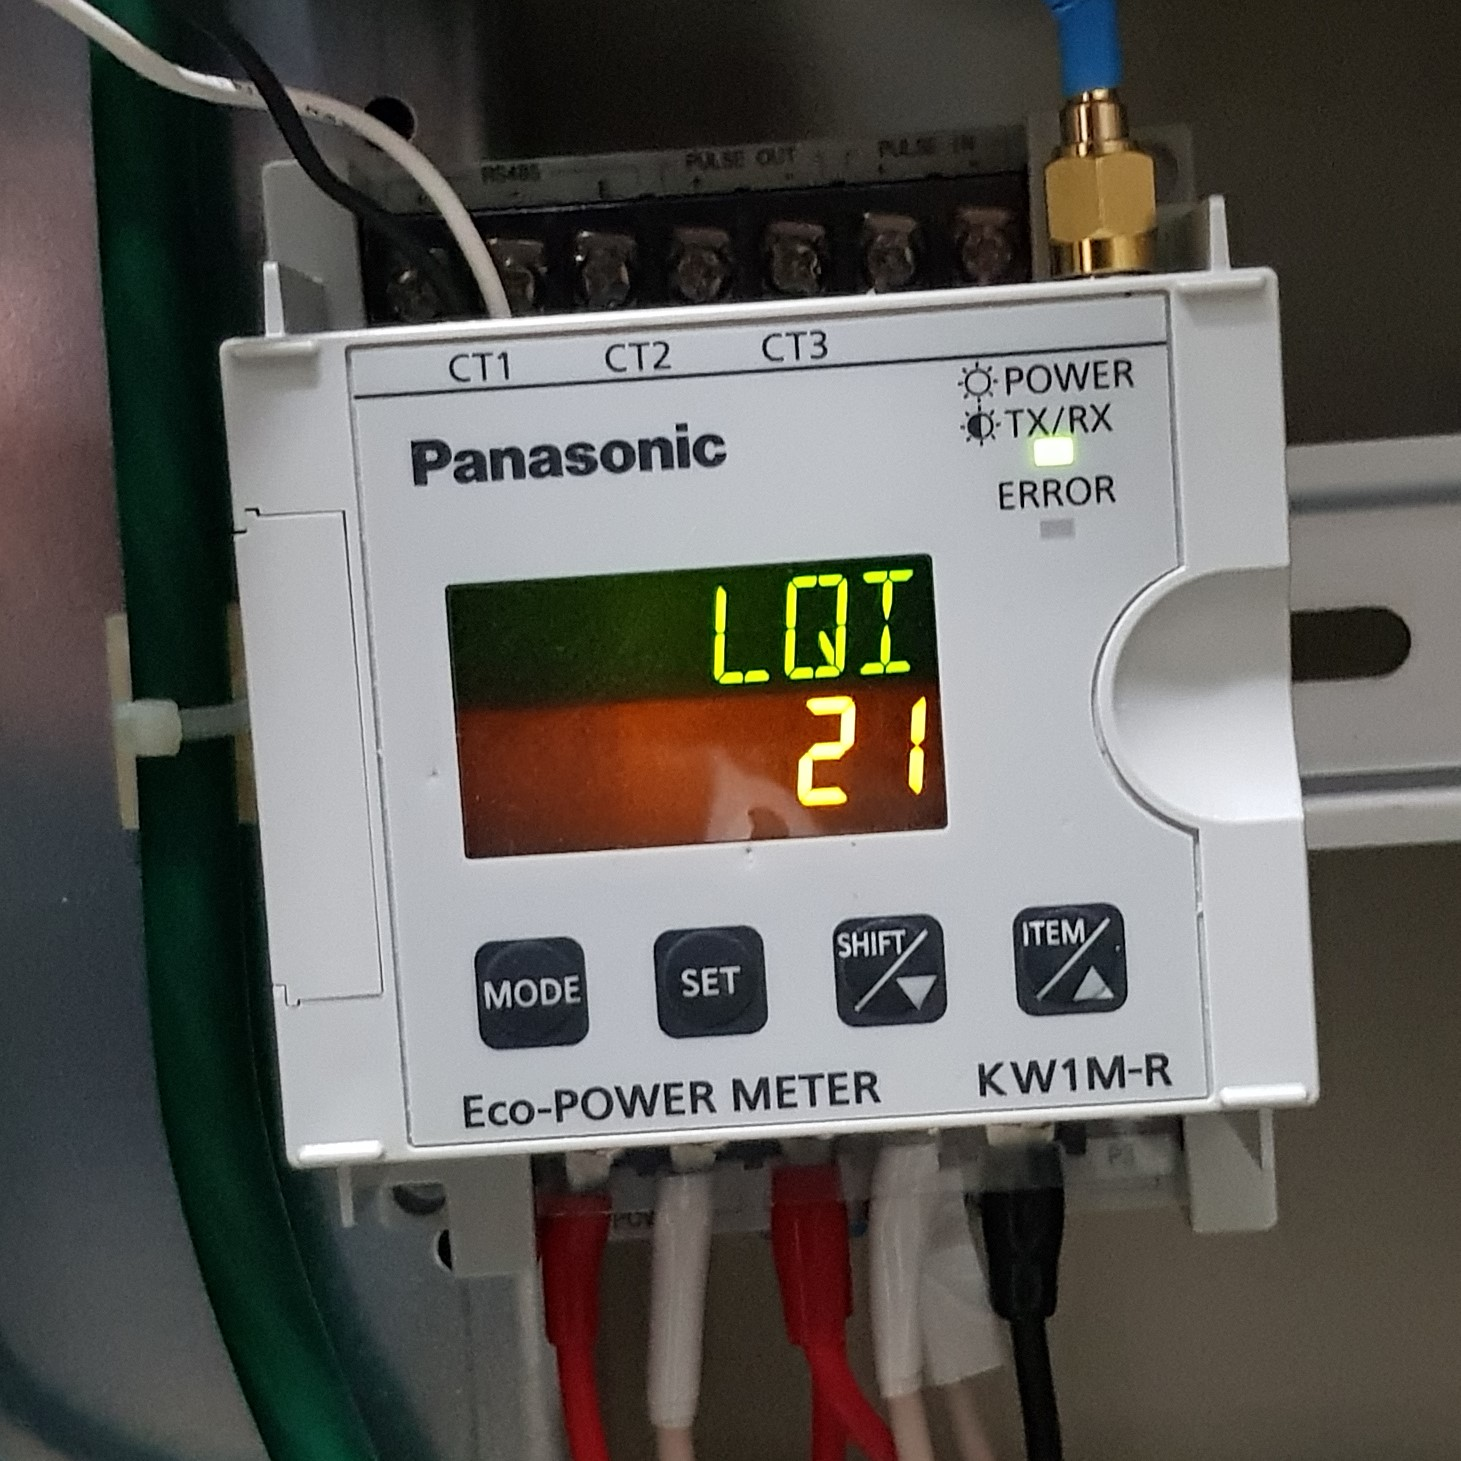
\includegraphics[width=\textwidth]{10f/1_2_slave}
        \caption{\small KW1M-R Slave Unit \\ (10F EPS-4)}
        \label{fig:s4_slave}
    \end{subfigure}
    \hfill
    \begin{subfigure}[b]{0.3\textwidth}
        \centering
        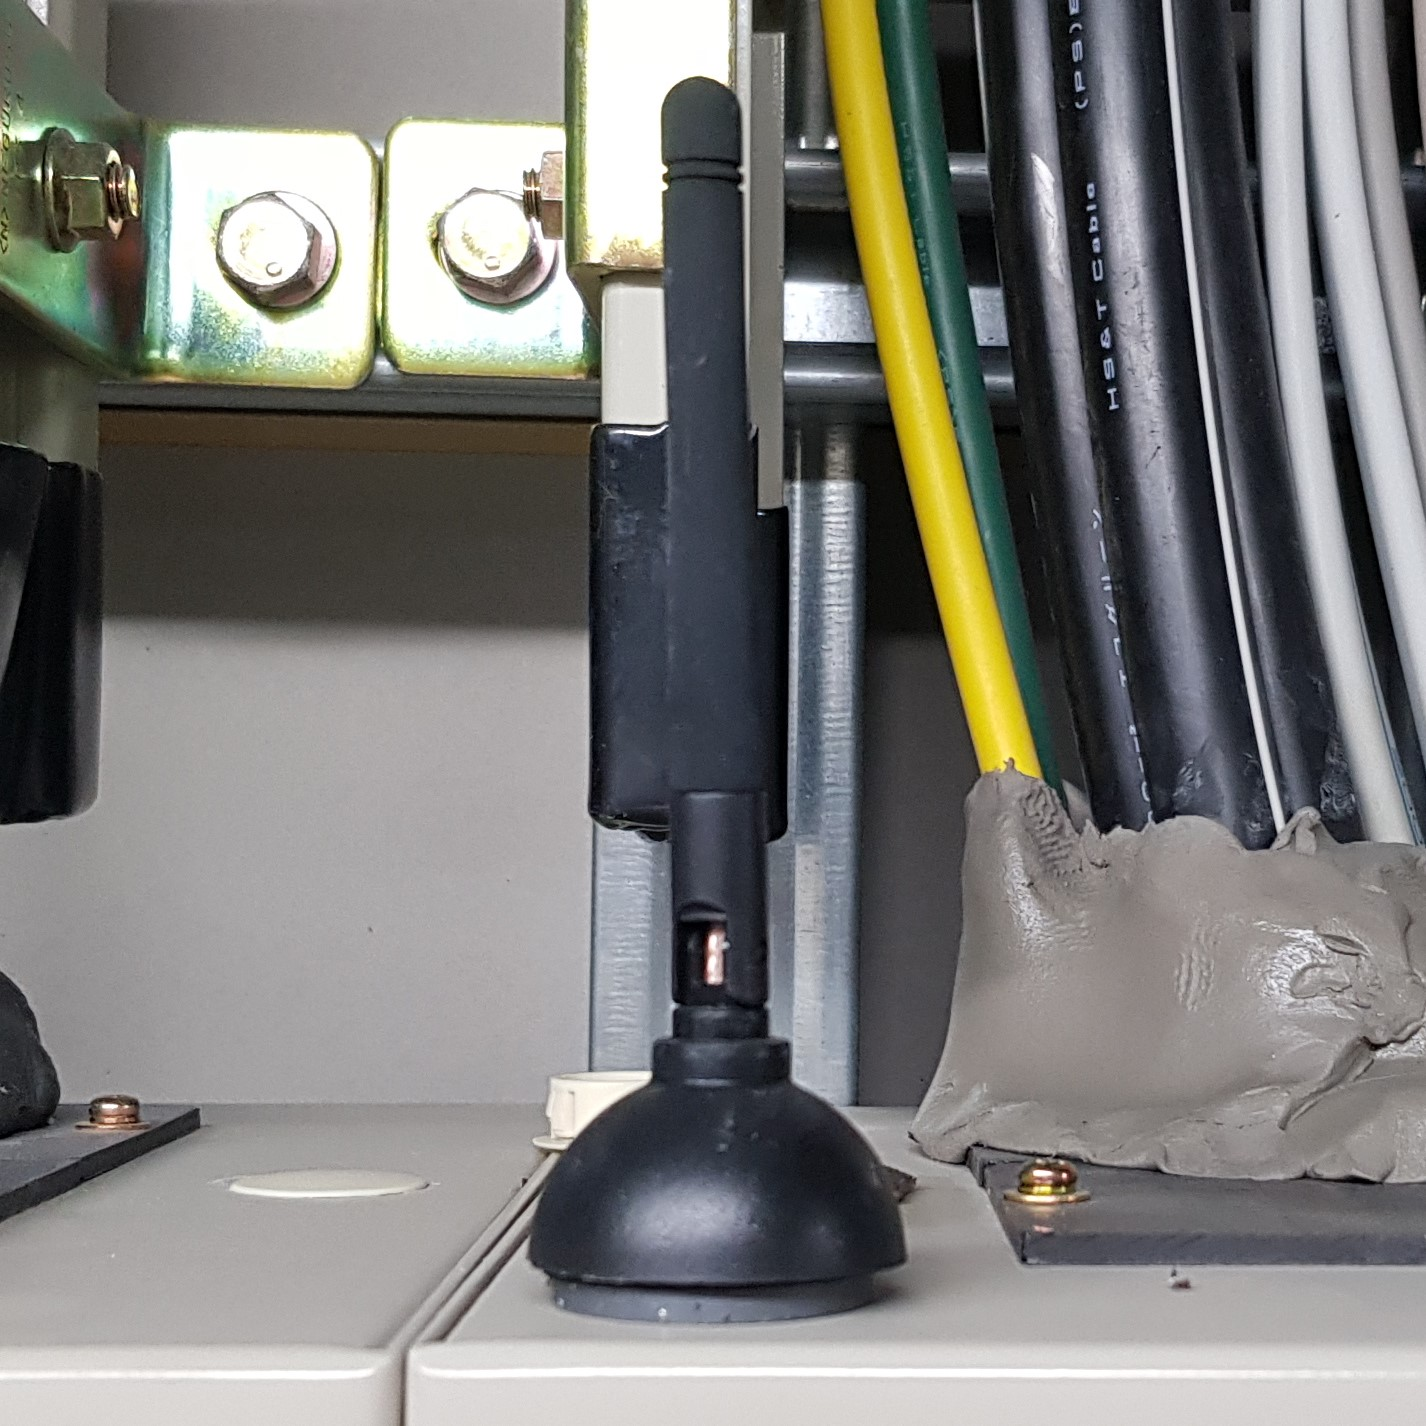
\includegraphics[width=\textwidth]{10f/1_3_antenna}
        \caption{\small Antenna connected to Slave Unit for transmission}
        \label{fig:s4_antenna}
    \end{subfigure}

    \begin{subfigure}[b]{0.3\textwidth}
        \centering
        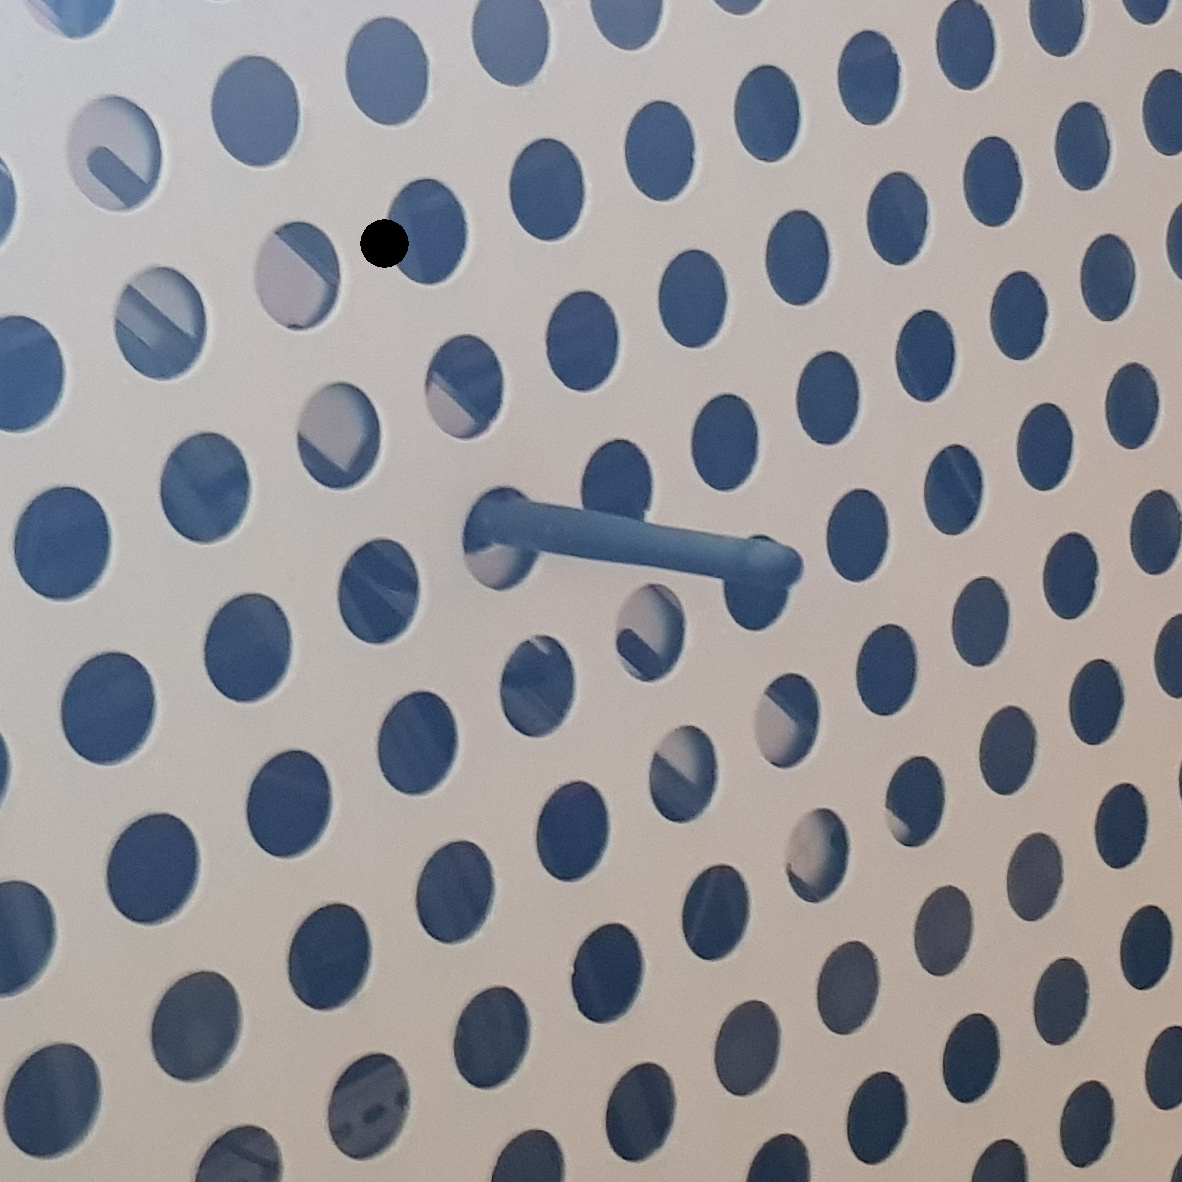
\includegraphics[width=\textwidth]{10f/2_1_repeater}
        \caption{Antenna of repeater (Hallway 10F)}
        \label{fig:s4_repeater}
    \end{subfigure}
    \hfill
    \begin{subfigure}[b]{0.3\textwidth}
        \centering
        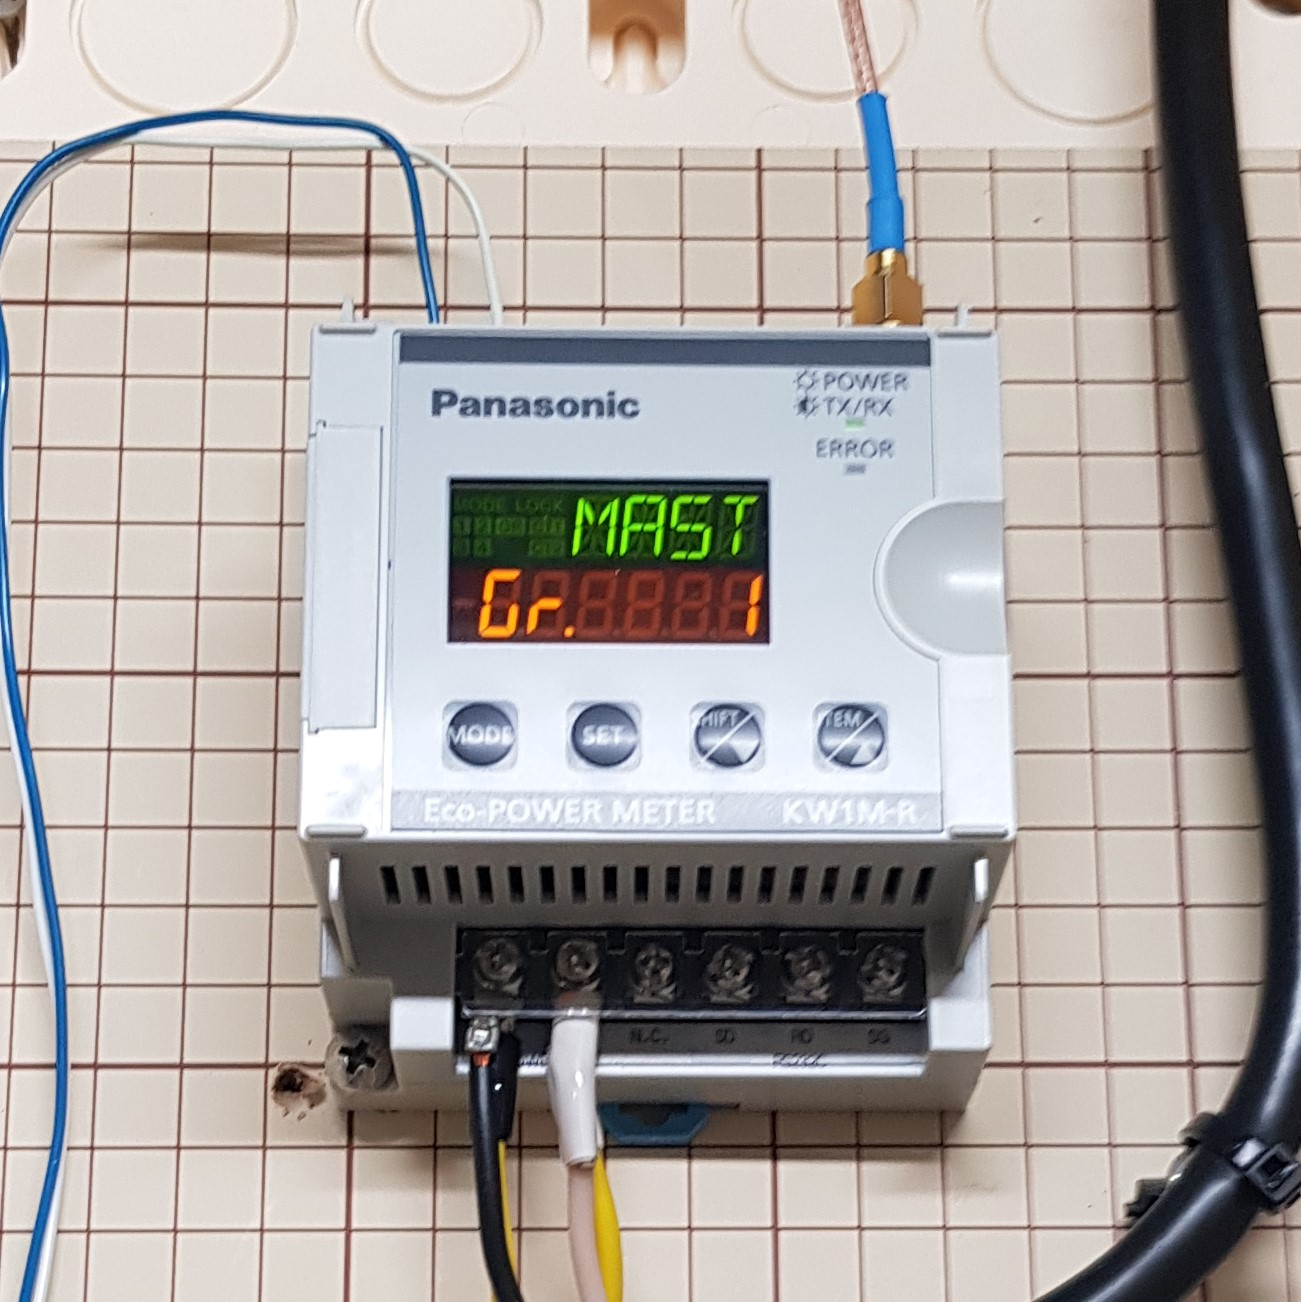
\includegraphics[width=\textwidth]{10f/2_2_master}
        \caption{KW1M-R Master Unit \\ (10F EPS-1)}
        \label{fig:s4_master}
    \end{subfigure}
    \hfill
    \begin{subfigure}[b]{0.3\textwidth}
        \centering
        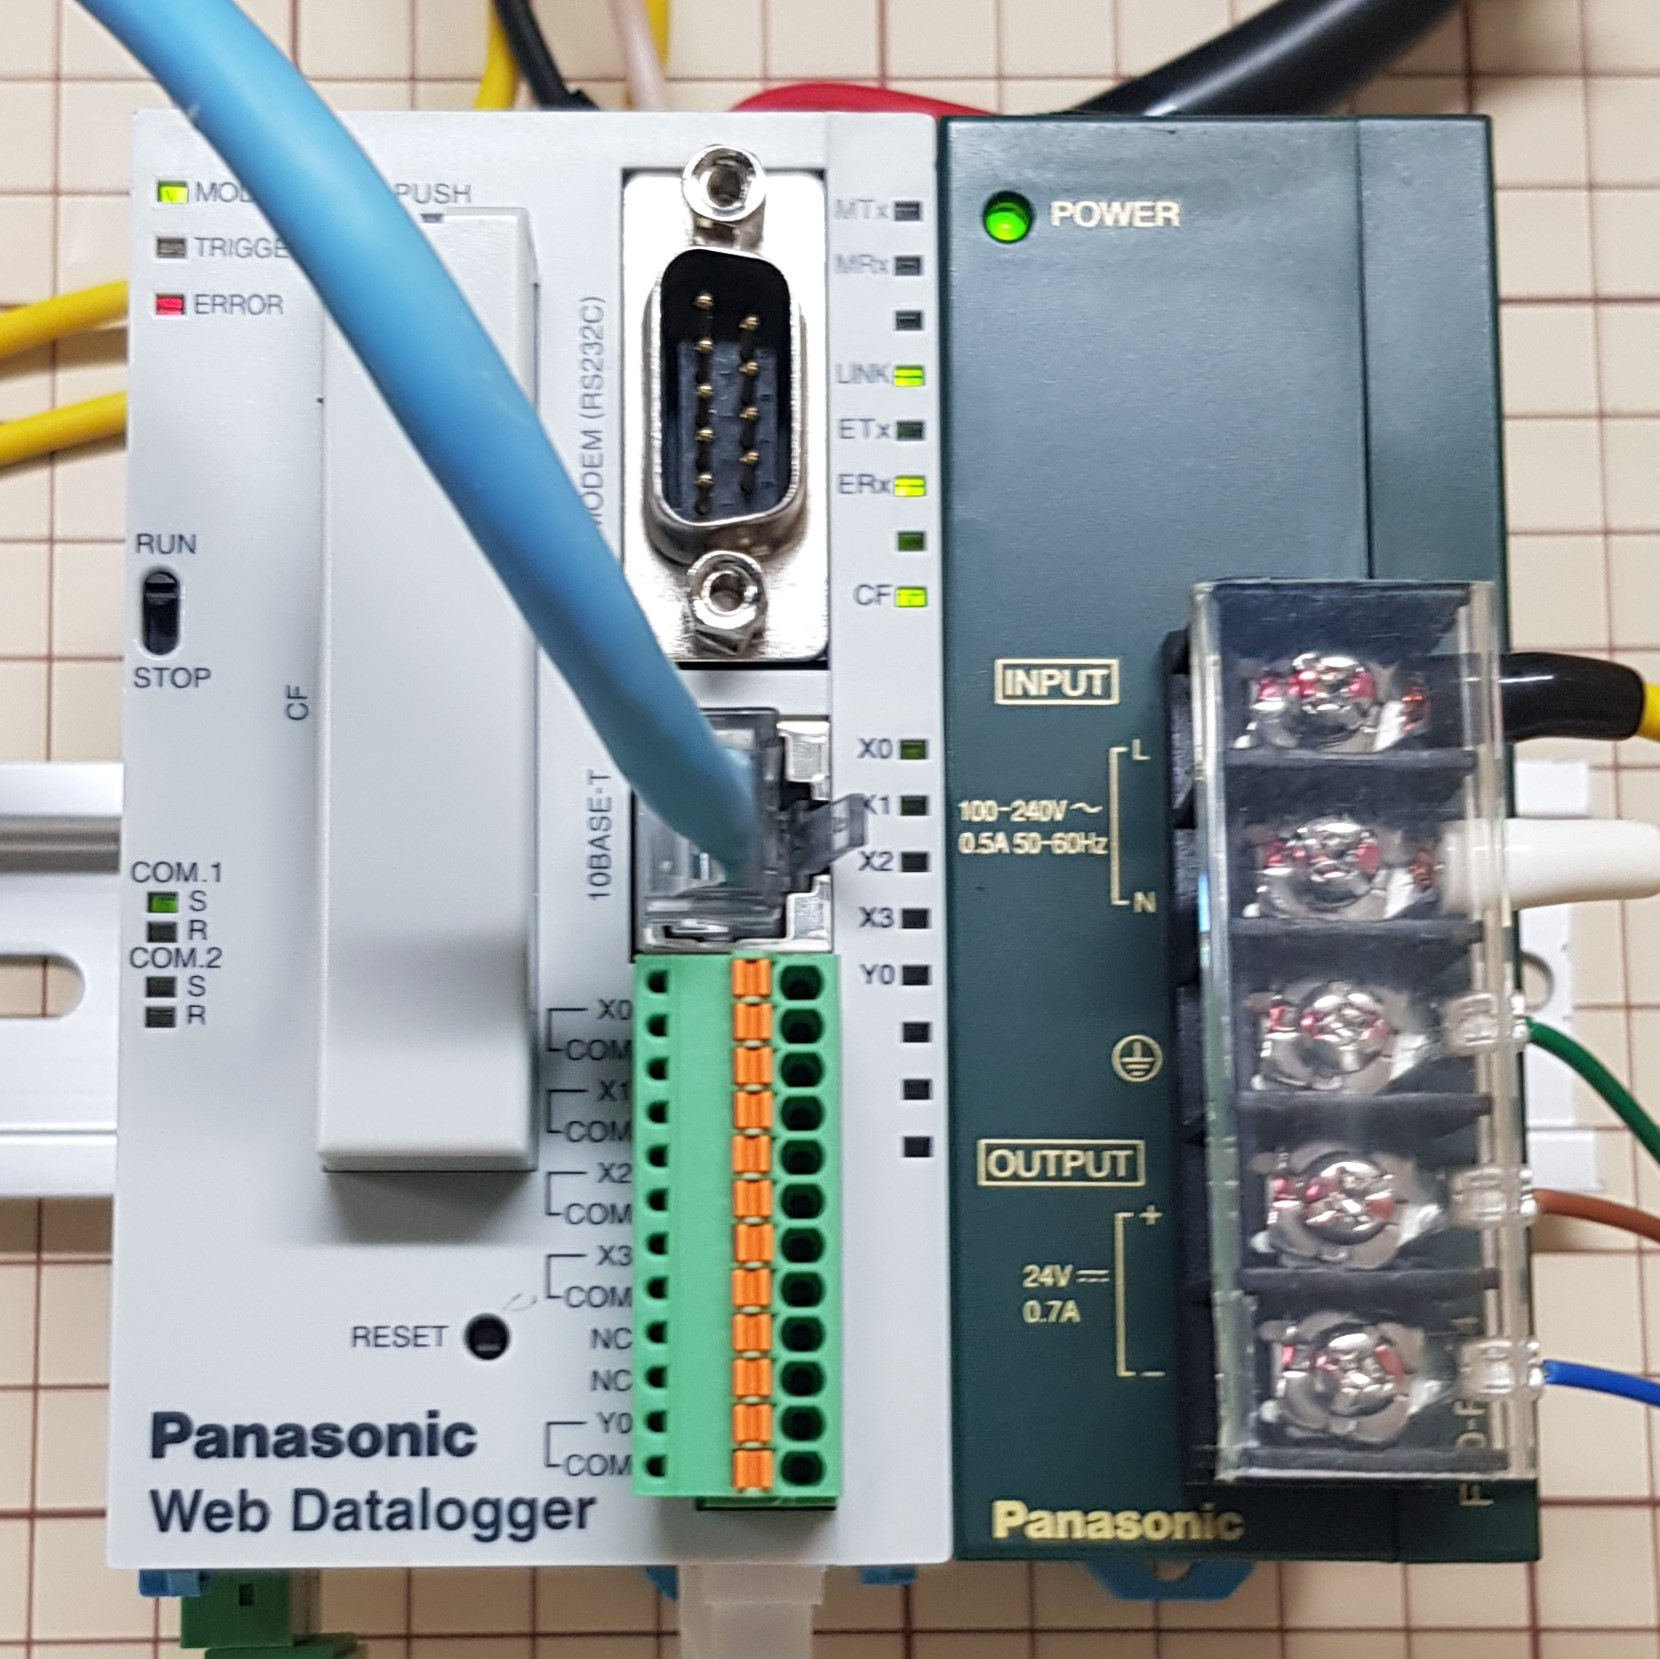
\includegraphics[width=\textwidth]{10f/2_3_dlu}
        \caption{Web Datalogger Unit \\(10F EPS-1) }
        \label{fig:s4_dlu}
    \end{subfigure}

    \caption{10F's components}
\end{figure}


Measurement unit (\ref{fig:s4_measure}) is dispersedly attached to the electric cables in various place around the 10th floor, assessing the electrical usage. 
The data collected from measurement unit is then passed through cable to the slave transmitter(\ref{fig:s4_slave}). 
Slave transmitter send data to its Master transmitter(\ref{fig:s4_master}) wirelessly with the help of repeater(\ref{fig:s4_repeater}). 
After the data reaches the master station, data is stored into the database using UDL (\ref{fig:s4_dlu}). 
Data is then visualized and shown on the webserver.figure \ref{fig:s4_location} shows the location of each device.

\begin{figure}[H]
    \centering
    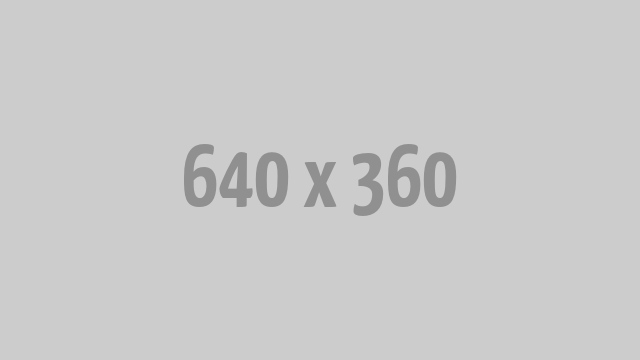
\includegraphics[width=0.5\textwidth]{place_holder}
    \caption{Location of each device.}
    \label{fig:s4_location}
\end{figure} 
